%%%%%%%%%%%%%%%%%%%%%%%%%%%%%%%%%%%%%%%%%%%%%%%%%%
%%%%		~~~~ EDITOR'S NOTE ~~~~
%%%%%%%%%%%%%%%%%%%%%%%%%%%%%%%%%%%%%%%%%%%%%%%%%%
%
% This is the PhD thesis of Laurens P. Stoop in LaTeX
%
% For the initial implementation big thanks to Douwe M. van Willigen.
% The original dissertation class was implemented by the TU Delft.
%
% This document is inteded to be a style guide to a nice and fancy LaTeX thesis.
%			- Comments are used to explain code (% sign)
%			- Make it your own by selecting only the things you want
%			- If in possible options you meet a couple of dots (...) more options are available (see documentation of pkg)
%
% Comments, remarks and more: email me at laurensstoop@protonmail.com
%
%%%%%%%%%%%%%%%%%%%%%%%%%%%%%%%%%%%%%%%%%%%%%%%%%%
%%%%	 	 ~~~~ END OF: EDITOR'S NOTE ~~~~
%%%%%%%%%%%%%%%%%%%%%%%%%%%%%%%%%%%%%%%%%%%%%%%%%%



%%%%%%%%%%%%%%%%%%%%%%%%%%%%
%%%%            ~~~~ Preamble ~~~~
%%%%%%%%%%%%%%%%%%%%%%%%%%%%

%% The document class dissertation is used
\documentclass[]{dissertation}

%% The thesis stylesheet, includes more package specifics
%%%%%%%%%%%%%%%%%%%%%%%%%%%%%%%%%%%%%%%%%%%%%%%%%%
%%%%		~~~~ EDITOR'S NOTE ~~~~
%%
%% This file contains the stylesheet
%% 
%% This is the PhD thesis of Laurens P. Stoop in LaTeX
%%                       - Comments, remarks and more: email me at laurensstoop@protonmail.com
%%
%%%%%%%%%%%%%%%%%%%%%%%%%%%%%%%%%%%%%%%%%%%%%%%%%%

%% For template only
\usepackage{lipsum}

%%%%%%%%%%%%%%%%%%%%%%%%%%%%%%%%%%%%%%%%%%%%%%%%%%
%%%% ~~~~ Extra package invocation & Settings

%% For acces to special signs
\usepackage{marvosym}


%% For access to written out month/year information & setting this
\usepackage{datetime}
\newdateformat{monthyeardate}{\monthname[\THEMONTH] \THEYEAR}

%% Create a list of acronyms.
\usepackage{acro}
% Set the acronyms in the PDF to link back to the acronym list
\acsetup{make-links=true}


%% Allow for the page-layout to be show explicit
\usepackage{layout}

%% For better TOC's
\usepackage{tocloft}

%% For making the parskip command work better
\usepackage[parfill]{parskip}

%% Neater font encoding
\usepackage[T1]{fontenc}

%% For setting space within document
\usepackage{setspace}


\usepackage{import}
%\usepackage[final]{changes}
%\usepackage{dblfloatfix}

%% To generate lipsum text
\usepackage{lipsum}
\usepackage{mdframed}

% For nicer subfigures
\usepackage{subcaption}

% for nicer non-forced page breaks
\usepackage{afterpage}

\usepackage{bm}


\usepackage[many]{tcolorbox}

% Package to provide a way to review
%       - gives TeXstudio access to the tools
%\usepackage{easyReview}

% for the cross-page table for the SIKS dissertation list
\usepackage{xltabular}
% for midrules within the SIKS dissertation list
\usepackage{booktabs}

\usepackage{csquotes}


%%%%%%%%%%%%%%%%%%%%%%%%%%%%%%%%%%%%%%%%%%%%%%%%%%
%%%% ~~~~ Left-opening pages

%% This would allow for opening on left page of chapters
%
% First option
%
% \makeatletter
% \renewcommand*\cleardoublepage{\clearpage\if@twoside
%        \ifodd\c@page \hbox{}\newpage\if@twocolumn\hbox{}%
%        \newpage\fi\fi\fi}
% \makeatother
%
% Other option
% This fixes the page to open chapters / parts on (i.e. not forced right)
% \csname @openrightfalse\endcsname

%%%%%%%%%%%%%%%%%%%%%%%%%%%%%%%%%%%%%%%%%%%%%%%%%%
%%%% ~~~~ Bibliography

%% Definition of the bibliography and related packages
% \usepackage[style=authoryear-comp,backend=biber,maxbibnames=10]{biblatex}
\usepackage[style=nature,backend=biber,maxbibnames=30]{biblatex}

%% For optional bibliography per chapter
%\usepackage{chapterbib}
%\setlength\bibitemsep{1.5\itemsep}
%\renewcommand*{\nameyeardelim}{\addcomma\space}


%%%%%%%%%%%%%%%%%%%%%%%%%%%%%%%%%%%%%%%%%%%%%%%%%%
%%%% ~~~~ Tikz settings

%% Getting Tikz
\usepackage{tikzscale}
\usepackage{tikz}

%% Tikz libraries
\usetikzlibrary{shapes,arrows,chains}

%\usepackage{pgfplots}
%\pgfplotsset{compat=newest}
%\pgfplotsset{plot coordinates/math parser=false}
\newlength{\fwidth}
\colorlet{lcnorm}{black}

% Better enumeration
%\usepackage[inline]{enumitem}



%%%%%%%%%%%%%%%%%%%%%%%%%%%%%%%%%%%%%%%%%%%%%%%%%%
%%%% ~~~~ Page tweaking

%% Remove the marginpar
\setlength{\marginparwidth}{0pt}


% Layout settings:
\renewcommand{\headrulewidth}{1.5pt}% 1.5pt header rule


%%%%%%%%%%%%%%%%%%%%%%%%%%%%%%%%%%%%%%%%%%%%%%%%%%
%%%% ~~~~ Figure tweaking

%% Small change to plot all figures with fbox, for better layout
\LetLtxMacro\latexincludegraphics\includegraphics % save the meaning of \includegraphics

% pass the image to \shadowbox
%\renewcommand{\includegraphics}[2][]{\fbox{\latexincludegraphics[#1]{#2}}}



%%%%%%%%%%%%%%%%%%%%%%%%%%%%%%%%%%%%%%%%%%%%%%%%%%
%%%% ~~~~ Subcript text

%% Change the behavior of subscript to textmode (without the amsmath spacing)
\begingroup\lccode`~=`!
\lowercase{\endgroup\def~}#1{_{\mathrm{#1}}}
\AtBeginDocument{\mathcode`!=\string"8000 }





%%%%%%%%%%%%%%%%%%%%%%%%%%%%%%%%%%%%%%%%%%%%%%%%%%
%%%% ~~~~ Table of Contents (TOC)
\makeatletter

\newcommand{\chaptoc}{
	\vspace{0.6cm}
	\startcontents[chaps]
	\begin{tcolorbox}[
		colframe=thumb\arabic{thumbcounter},
		width=\linewidth,
		enhanced,
		top=10pt,
		bottom=10pt,
		nobeforeafter,
		outer arc=0pt,
		arc=0pt,
		boxrule=1.2pt,
		colback=white,
		overlay={
			\node[anchor=west,fill=white,inner xsep=6pt, text=thumb\arabic{thumbcounter}]
			at ([xshift=10pt]frame.north west)
			{\textbf{Contents}};
		}
		]
		\printcontents[chaps]{}{1}{}
	\end{tcolorbox}
	\vspace{2cm}}



%%%%%%%%%%%%%%%%%%%%%%%%%%%%%%%%%%%%%%%%%%%%%%%%%%
%%%% ~~~~ Styling the Part

%% Make changes to the part so that the contents end up on the titlepages
\let\LaTeXStandardPart\part%
\newcommand{\unstarredpart@@noopt}[1]{%
	\unstarredpart@@opt[#1]{#1}%
}%

\newcommand{\unstarredpart@@opt}[2][]{%
%	\cleardoublepage% (For clearing content before!!) Original
        \clearpage% (For clearing content before!!!)
	\begingroup%
	\let\newpage\relax%
	\LaTeXStandardPart[#1]{#2}%
	\endgroup%
}%

\newcommand{\starredpart}[1]{%
	\LaTeXStandardPart*{#1}%
}%

\newcommand{\unstarredpart}{%
	\@ifnextchar[{\unstarredpart@@opt}{\unstarredpart@@noopt}%
}%

\renewcommand{\part}{%
	\@ifstar{\starredpart}{\unstarredpart}%
}%

\makeatother



%% Define the toc colors for the parts, and add the horizontal lines
\renewcommand{\cftpartfont}{\hypersetup{linkcolor=thumb\arabic{colorcounter}}}
\renewcommand{\cftpartpresnum}{\hypersetup{linkcolor=thumb\arabic{colorcounter}}}

\titlecontents{part}%
[0pt]{\stepcounter{colorcounter}\color{thumb\arabic{colorcounter}}\bfseries\large\protect\addvspace{10pt}\titlerule[1pt]\addvspace{1.3ex}}
{}{\partname~}
{\hfill\contentspage}%
[\addvspace{0.7ex} {\titlerule[1pt]} \addvspace{5pt}]%

\renewcommand{\cftchapfont}{\bfseries\hypersetup{linkcolor=thumb\arabic{colorcounter}}}
\renewcommand{\cftchappagefont}{\bfseries\color{thumb\arabic{colorcounter}}}

\renewcommand{\thepart}{\color{thumb\arabic{colorcounter}}\Roman{part}} % Adjust the color of the part as well

\DeclareRobustCommand{\IncCLR}{\protect\stepcounter{colorcounter}}

\newcounter{thumbcounter}
\newcounter{colorcounter}



%% Include the acronyms definition
%%%%%%%%%%%%%%%%%%%%%%%%%%%%%%%%%%%%%%%%%%%%%%%%%%
%%%%		~~~~ EDITOR'S NOTE ~~~~
%%%%%%%%%%%%%%%%%%%%%%%%%%%%%%%%%%%%%%%%%%%%%%%%%%
%
% This file contains the fancy definition of acronyms
%                       - requires a full compilation cycle to work properly
%                       - when defined here, the handle can be used in text with \ac{<handle>}
%
% This is the PhD thesis of Laurens P. Stoop in LaTeX
%                       - Comments, remarks and more: email me at laurensstoop@protonmail.com
%
%%%%%%%%%%%%%%%%%%%%%%%%%%%%%%%%%%%%%%%%%%%%%%%%%%
%%%%	 	 ~~~~ END OF: EDITOR'S NOTE ~~~~
%%%%%%%%%%%%%%%%%%%%%%%%%%%%%%%%%%%%%%%%%%%%%%%%%%



%%%%%%%%%%%%%%%%%%%%%%%%%%%%
%%%%            ~~~~ Example ~~~~
%%%%%%%%%%%%%%%%%%%%%%%%%%%%
%
%
% For a given handle, an acronym's full definition can be provided with:
%        \DeclareAcronym{<handle>}{
%                short=<acronym>,
%                long=<full definition>,
%        }
%
% In text then used with \ac{<handle>}
%       - Full form first time (forced with \acf{<handle>} )
%       - Short form after this (forced with \acs{<handle>} )
%       - Long form  forced with \acl{<handle>}
% If needed specifically

%% Example used in the Introduction
\DeclareAcronym{eu}{
        short=EU,
        long=European Union
}




%% Author and Title for use everywhere
\title[or an approach from multiple fields]{AC\lightning DC}
\author{Laurens~Persijn}{Stoop}



\begin{document}
%% strong use of \include{file} to reduce compilation time in draft stage
%               - tex-files of chapters are located in (sub-)folders (FrontMatter, MainMatter, BackMatter)
%               - for filling Lorem-Ipsum is used with the \lipsum[num-num] command




%%%%%%%%%%%%%%%%%%%%%%%%%%%%
%%%%            ~~~~ FrontMatter ~~~~
%%%%%%%%%%%%%%%%%%%%%%%%%%%%
%
% This includes everything before the introduction
%               - Cover
%               - Titlepages [required]
%               - Table of Contents [required]
%               - Prologue
%               - Glossary or list of acronyms
%
% Some PhD include the following at the begining instead of in the backmatter
%               - Summary  [required]
%               - Samenvatting  [required]
%               - Acknowledgements
%
% The order of these chapters, of the content is not 100% set in stone, after the cover and title-pages, there is some variation

%% Use Arabic numerals for the page numbers of the chapters.
\pagenumbering{roman}

%% Use Frontmatter to set some styleproperties
\frontmatter


%% Cover
%%%%%%%%%%%%%%%%%%%%%%%%%%%%%%%%%%%%%%%%%%%%%%%%%%
%%%%		~~~~ EDITOR'S NOTE ~~~~
%%%%%%%%%%%%%%%%%%%%%%%%%%%%%%%%%%%%%%%%%%%%%%%%%%
%
% This file contains the cover pages these are rather basic and depend on the imagery used
%                       - a change to your own cover image is needed
%                       - be mindfull of some tweaking
%
% This is the PhD thesis of Laurens P. Stoop in LaTeX
%                       - Comments, remarks and more: email me at laurensstoop@protonmail.com
%
%%%%%%%%%%%%%%%%%%%%%%%%%%%%%%%%%%%%%%%%%%%%%%%%%%
%%%%	 	 ~~~~ END OF: EDITOR'S NOTE ~~~~
%%%%%%%%%%%%%%%%%%%%%%%%%%%%%%%%%%%%%%%%%%%%%%%%%%



%%%%%%%%%%%%%%%%%%%%%%%%%%%%
%%%%            ~~~~ Cover ~~~~
%%%%%%%%%%%%%%%%%%%%%%%%%%%%

%% Titlepage enviroment is used for some commands
\begin{titlepage}

        %% This can be used to set a background image (for instance a base colour)
        %               - the oversize (1.07) is used to make sure that the image bleeds into the side
        %               - opacity is something to set
        \tikz[remember picture,overlay] \node[opacity=0.8,inner sep=0pt] at (current page.center){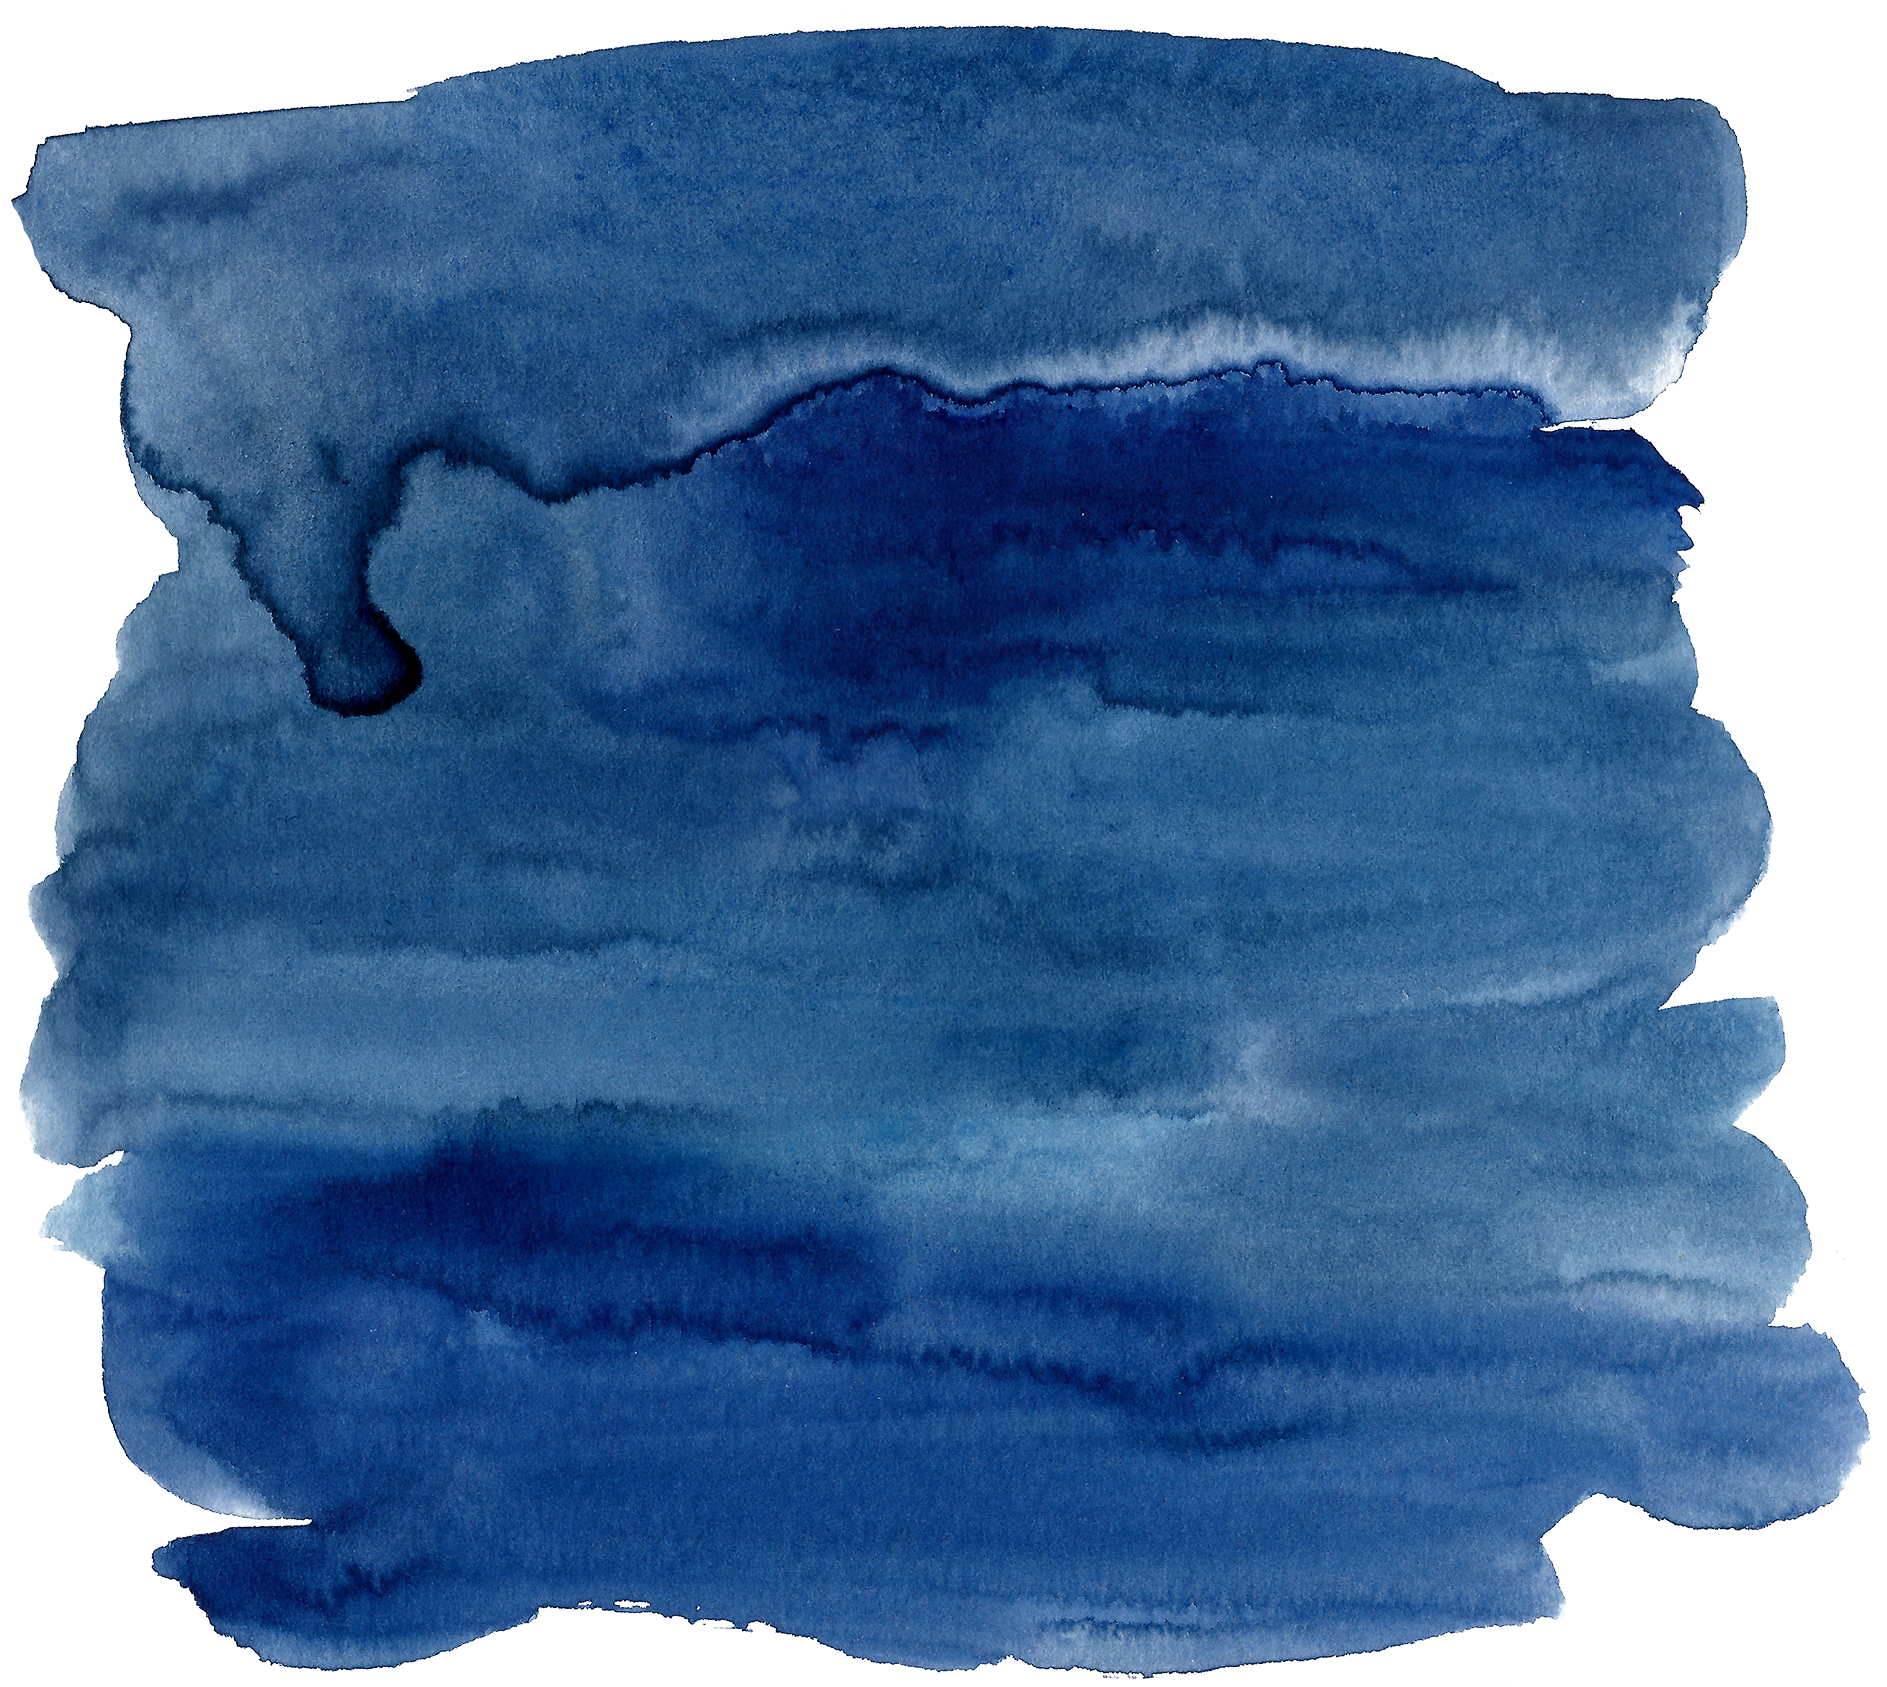
\includegraphics[width=1.07\paperwidth,height=1.07\paperheight]{FrontMatter/Cover/CoverBackground}};


        %% we center all text
        \begin{center}


        %% Text color is changed for readability
        %               - options are: white/black
        %               - additional colours are defined in the stylesheet
        \color{white}

        %% Print the title (ussually only the title is given)
        %               - Explicit control over fontsize is used to make it fit nicely
        {\makeatletter
                \largetitlestyle\fontsize{1.2cm}{13cm}\selectfont\@title
                \makeatother}

        %% Print the optional subtitle
        %               - Explicit control over fontsize is used to make it fit nicely
        {\makeatletter
                \ifx\@subtitle\undefined\else
                \bigskip
                \largetitlestyle\fontsize{0.8cm}{13cm}\selectfont\@subtitle
                \fi
                \makeatother}


        %% Additional whitespace for ease of eye
        \vfill


        %% This can be used to set a foreground image
        %               - Ussually some tweaking with vertical space is needed to place it exactly
        \begin{figure}[H]
%        	\vspace*{-3.5cm}
        	\makebox[\linewidth]{
                		\includegraphics[width=0.6\textwidth, clip, trim={0cm 0cm 0cm 0cm}]{FrontMatter/Cover/Cover}
                	}
%        	\vspace*{1.0cm}
        \end{figure}



        %% Additional whitespace for ease of eye
        \vspace*{2\bigskipamount}


         %% Text color is changed for readability
        \color{white}

        %% Print the name of the author.
        {\makeatletter
                \largetitlefont\Large\bfseries
                \largetitlestyle\fontsize{24}{13cm}\selectfont\@firstname~\@lastname
                \makeatother}


        %% Additional whitespace for ease of eye
        \vspace*{2\bigskipamount}
        \end{center}


\end{titlepage}

%% Titlepage
%%%%%%%%%%%%%%%%%%%%%%%%%%%%%%%%%%%%%%%%%%%%%%%%%%
%%%%		~~~~ EDITOR'S NOTE ~~~~
%%%%%%%%%%%%%%%%%%%%%%%%%%%%%%%%%%%%%%%%%%%%%%%%%%
%
% This file contains the title pages in the required Utrecht University format
%                       - formal required text fields are included
%                       -
%
% This is the PhD thesis of Laurens P. Stoop in LaTeX
%                       - Comments, remarks and more: email me at laurensstoop@protonmail.com
%
%%%%%%%%%%%%%%%%%%%%%%%%%%%%%%%%%%%%%%%%%%%%%%%%%%
%%%%	 	 ~~~~ END OF: EDITOR'S NOTE ~~~~
%%%%%%%%%%%%%%%%%%%%%%%%%%%%%%%%%%%%%%%%%%%%%%%%%%



%%%%%%%%%%%%%%%%%%%%%%%%%%%%
%%%%            ~~~~ Titlepage ~~~~
%%%%%%%%%%%%%%%%%%%%%%%%%%%%

% This enviroment is called as the titlepage is spread over 4 pages and therefore required
\begin{titlepage}



%%%%%%%%%%%%%%%%%%%%%%%%%%%%
%%%%            ~~~~ Page 1 (base titlepage) ~~~~
%%%%%%%%%%%%%%%%%%%%%%%%%%%%

        %% Centered title page, first page always is without style elements
	\begin{center}

		%% Some whitespace at the top.
                \vspace*{2\bigskipamount}

                %% Print the title (bold and big)
                % To make the title fit better it could be benificial to change \Huge to \huge, \LARGE or even \Large
                {\makeatletter
                        \titlestyle\bfseries\Huge\@title
                        \makeatother}

                %% Print the optional subtitle.
                % To make the subtitle fit better it could be benificial to change \LARGE to \Large or \large
                {\makeatletter
                        \ifx\@subtitle\undefined\else
                        \bigskip
                        \titlefont\titleshape\LARGE\@subtitle
                        \fi
                        \makeatother}

                %% Fill out the page
                \vfill

                %% Print the author (bold is traditional)
                % To make the name fit better it could be benificial to change \LARGE to \Large or \large
                {\makeatletter
                        \titlestyle\bfseries\LARGE\@firstname~{\titleshape\@lastname}
                        \makeatother}

                %% Extra whitespace at the bottom.
                \vspace*{4\bigskipamount}


	\end{center}


%%%%%%%%%%%%%%%%%%%%%%%%%%%%
%%%%            ~~~~ Page 2 (verso with CIP data) ~~~~
%%%%%%%%%%%%%%%%%%%%%%%%%%%%

% Any unrelevant lines should be commented or removed

        %% Go to new page by forcing to clear all floats
	\clearpage

        %% Empty page style as we don't want numbers
	\thispagestyle{empty}

                %% The information is traditionally listed near the bottom
                \vspace*{\fill}

                %% Inclusion of logos of research schools (not sure if allowed)
               	\begin{center}
                        \includegraphics[height=0.5in]{FrontMatter/Logos/nwo}
                        \hspace{2em}
                        \includegraphics[height=0.5in]{FrontMatter/Logos/sikskleur}
                \end{center}
                \medskip

                %% Include the following lines (or something similair) if the dissertation is part of a series
                \noindent SIKS Dissertation Series No. XXX \\
                The research reported in this thesis has been carried out under the auspices of SIKS, the Dutch Research School for Information and Knowledge Systems.

                %% Additional whitespace for ease of eye
             	\vspace{\bigskipamount}

                %% Listing of book information (ISBN recommended, printerlisting ussualy required by company, credit for cover)
               	\noindent
               	\begin{tabular}{@{}p{0.2\textwidth}@{}p{0.8\textwidth}}
          		\textit{ISBN:} &  000-00-0000-000-0 \\[\medskipamount]
                	\textit{Printed by:} & Johannes Gutenberg \\[\medskipamount]
                	\textit{Cover by:} & Beautiful cover art that captures the entire content of this thesis in a single illustration.
                \end{tabular}

                %% Additional whitespace for ease of eye
                \medskip

                %% Statement if 100\% recycled paper is used
                \noindent This dissertation was printed on 100\% recycled paper in an effort to minimize the enviromental footprint.

                %% Additional whitespace for ease of eye
             	\vspace{\bigskipamount}

                %% Copyright information
                % Could also be inserted manually around the change of the calander year
               	\noindent Copyright \textcopyright\ \the\year{} by {\makeatletter\@firstname~\@lastname \makeatother}

               %% More restricting copyright statement
               % This is very relevant if part is unpublished
               All rights reserved. No part of this publication may be reproduced, stored in a retrieval system or transmitted in any form without the written permission of the copyright owner.

                % At the UU it's required to publish your dissertation online
                % Be aware that this location is subject to change
                \noindent An electronic version of this dissertation is available at \url{https://dspace.library.uu.nl/}.





%%%%%%%%%%%%%%%%%%%%%%%%%%%%
%%%%            ~~~~ Page 3 (Formal titlepage) ~~~~
%%%%%%%%%%%%%%%%%%%%%%%%%%%%

%% NB: contents here are dictated by regulations; CHECK THEM

        %% Go to new page by forcing to clear all floats
        \clearpage

        %% Empty page style as we don't want numbers
        \thispagestyle{empty}

        %%
	\begin{center}

		%% some whitespace at the top
		\vspace*{2\bigskipamount}

		%% Print the title (original language).
		{\makeatletter
			\titlestyle\bfseries\Huge\@title
			\makeatother}

		%% Print the optional subtitle.
		{\makeatletter
			\ifx\@subtitle\undefined\else
			\bigskip
			\titlefont\titleshape\LARGE\@subtitle
			\fi
			\makeatother}

                %% Flush the rest of the page to the bottom
		\vfill

		%% Apart from the names and dates, the following text is dictated by the doctorol degree regulations

                %% If original title in not-dutch, provide it in Dutch.
		{\LARGE\titlefont\bfseries Titel in het Nederlands}

                %% Also provide a dutch optional sub-title
                {\Large\titlefont\titleshape Sub-titel in het Nederlands}

                %% Required to state that it includes a summary
                % in Dutch if body not in Dutch
                % in English if body in Dutch
                (met een samenvatting in het Nederlands)

                %% Include some whitespace
		\bigskip
		\bigskip

                %% Required text by the doctoral degree regulations
                % NB: be very mindfull of the lower case lettering used!!!
                % NB: basically; do not change this bit
		ter verkrijging van de graad van doctor aan de Universiteit Utrecht

		op gezag van de rector magnificus, prof.dr.\ H.R.B.M.~Kummeling,

		ingevolge het besluit van het college voor promoties

		in het openbaar te verdedigen

                %% Change to relevant date for defense
                % written as: dayofweek(text) date(number) month(text)  year(number)
                % if in the morning use: des ochtends te XX.XX uur (use 12-hour format)
                % if in the afternoon use: des middags te XX.XX uur (use 12-hour format)
                op woensdag 5 april 2023  des ochtends te 10.30 uur%/des middags te 4.15 uur

                %% Include some whitespace
		\bigskip
		\bigskip

		door

                %% Include some whitespace
		\bigskip
		\bigskip

		%% Print the full name of the author.
		{\makeatletter
		\Large\titlefont\bfseries\@firstname~{\titleshape\@lastname}
		\makeatother}

                %% Include some whitespace
		\bigskip
		\bigskip

                %% Change to relevant date of birth and town
                % NB: include country if not born in the Netherlands
       		geboren op 5 april 2023 te Utrecht

		%% Extra whitespace at the bottom.
		\vspace*{2\bigskipamount}

	\end{center}




%%%%%%%%%%%%%%%%%%%%%%%%%%%%
%%%%            ~~~~ Page 4 (co-promotor listing) ~~~~
%%%%%%%%%%%%%%%%%%%%%%%%%%%%

%% NB: contents here are dictated by regulations; CHECK THEM

        %% Go to new page by forcing to clear all floats
        \clearpage

        %% Empty page style as we don't want numbers
        \thispagestyle{empty}

	%% List the (co-)promotors.
        % NB: Only use the title + initials + lastname
	\begin{tabular}{ll}
		Promotoren:           & Prof.\,dr.\ A.B.C.D.~Fancy \\[0.1cm]
                                                & Prof.\,dr.\ E.F.~Pants \\[0.1cm]
		Copromotoren:      & dr.\ G.H.~Twinkle \\[0.1cm]
                                                & Prof.\,dr.\,ir.\ I.J.~Toes
	\end{tabular}

        %% Flush the rest of the information to the bottom
        \vfill

        %% If Joint Doctorate, then uncomment below
        \noindent The degree is awareded as part of a Joint Doctorate with AAAAAAAA Univeristy.

     	%% Extra whitespace at the bottom.
        \vspace*{2\bigskipamount}

        %% Example of a financial support statement
        \noindent This work was support by the research project ACDC-ESM, which was financed by the Netherlands Organisation for Scientific Research under grant number 647.003.005 and supported by the stakeholders TenneT TSO B.V. and the Royal
        Netherlands Meteorological Institute.


\end{titlepage}




%% Table of Contents
%       - Set depth of ToC  at this point to 1
%       - Start all counters after the ToC
\setcounter{tocdepth}{1}
\tableofcontents
\startcontents


%% Print the acronym chapter here
\printacronyms



%% Dedication setting
%       - The (optional) dedication can be used to thank someone or display a significant quotation.
%       - a empty & clear page is needed
\clearpage
\thispagestyle{empty}
\dedication{\epigraph{Science is a wonderful thing \\ if one does not have to earn one's living at it.}{Albert Einstein}}





%% Prologue or preface
%%%%%%%%%%%%%%%%%%%%%%%%%%%%%%%%%%%%%%%%%%%%%%%%%%
%%%%		~~~~ EDITOR'S NOTE ~~~~
%%%%%%%%%%%%%%%%%%%%%%%%%%%%%%%%%%%%%%%%%%%%%%%%%%
%
% This file contains the optional preface of the dissertation
%                       - If included, it's recommended to keep it to 1.5 pages maximum.
%                       - Stylistically the preface is signed & dated
%
% This is the PhD thesis of Laurens P. Stoop in LaTeX
%                       - Comments, remarks and more: email me at laurensstoop@protonmail.com
%
%%%%%%%%%%%%%%%%%%%%%%%%%%%%%%%%%%%%%%%%%%%%%%%%%%
%%%%	 	 ~~~~ END OF: EDITOR'S NOTE ~~~~
%%%%%%%%%%%%%%%%%%%%%%%%%%%%%%%%%%%%%%%%%%%%%%%%%%



%%%%%%%%%%%%%%%%%%%%%%%%%%%%
%%%%            ~~~~ Preface ~~~~
%%%%%%%%%%%%%%%%%%%%%%%%%%%%

%% FrontMatter chapters are unlabeled, but part of the ToC
\chapter*{Preface}
% We add it to the ToC
\addcontentsline{toc}{chapter}{Preface}
% We set the header text
\setheader{Preface}

\emph{Preface goes here. This chapter is optional.}

%% Dumps Lorem-Ipsum
\lipsum[42-49]


%% Automatic signature
%       - change to static information if wanted
%       - italics are normally used
\begin{flushright}
{\makeatletter\itshape
    \@firstname\ \@lastname \\
    Utrecht, \monthyeardate\today
\makeatother}
\end{flushright}









%%%%%%%%%%%%%%%%%%%%%%%%%%%%
%%%%            ~~~~ MainMatter ~~~~
%%%%%%%%%%%%%%%%%%%%%%%%%%%%
%
% This includes at its core the following
%               - Introduction
%               - Publishable chapters;
%                       - here structured in multiple Parts
%               - Conclusion
%
% The location of the bibliography should be considered. This could be for:
%               - each seperate chapter (paper)
%               - each part
%               - Only once, near the end
%
%% Main Matter style settings
% Use Arabic numerals for the page numbers of the chapters.
\pagenumbering{arabic}
% caller for the general style definitions
\mainmatter
% Turn on thumb indices.
\thumbtrue



%%%%%%%%%%%%%%
%%      ~~~~ PART 0 ~~~~
%%%%%%%%%%%%%%
%
%% Set the Part name and properties
%\stepcounter{thumbcounter}
%\setcounter{colorcounter}{1}
%\part[\color{thumb\arabic{thumbcounter}}Introduction]{Introduction}\label{part:intro}
%\chaptoc

%% Introduction
%%%%%%%%%%%%%%%%%%%%%%%%%%%%%%%%%%%%%%%%%%%%%%%%%%
%%%%		~~~~ EDITOR'S NOTE ~~~~
%%%%%%%%%%%%%%%%%%%%%%%%%%%%%%%%%%%%%%%%%%%%%%%%%%
%
% This file contains the introduction
%
% This is the PhD thesis of Laurens P. Stoop in LaTeX
%                       - Comments, remarks and more: email me at laurensstoop@protonmail.com
%
%%%%%%%%%%%%%%%%%%%%%%%%%%%%%%%%%%%%%%%%%%%%%%%%%%
%%%%	 	 ~~~~ END OF: EDITOR'S NOTE ~~~~
%%%%%%%%%%%%%%%%%%%%%%%%%%%%%%%%%%%%%%%%%%%%%%%%%%



%%%%%%%%%%%%%%%%%%%%%%%%%%%%
%%%%            ~~~~ Introduction ~~~~
%%%%%%%%%%%%%%%%%%%%%%%%%%%%

\chapter{Introduction}\label{ch:Introduction}

This is a introduction chapter explaining the scientific and technical questions that are currently unsolved.

This line is merely intended to use as a reference to some acronyms used in the main text like \ac{eu} and when used again \ac{eu}.

%% Dumps Lorem-Ipsum
\lipsum[1]

\section{Some context}
%% Dumps Lorem-Ipsum
\lipsum[2-4]




%% Overview of contributions of the articles used
%%%%%%%%%%%%%%%%%%%%%%%%%%%%%%%%%%%%%%%%%%%%%%%%%%
%%%%		~~~~ EDITOR'S NOTE ~~~~
%%%%%%%%%%%%%%%%%%%%%%%%%%%%%%%%%%%%%%%%%%%%%%%%%%
%
% This file contains the Overview of contributions
%                       - this is optional
%                       - more commonly used when many collaborative scientific works are used
%
% This is the PhD thesis of Laurens P. Stoop in LaTeX
%                       - Comments, remarks and more: email me at laurensstoop@protonmail.com
%
%%%%%%%%%%%%%%%%%%%%%%%%%%%%%%%%%%%%%%%%%%%%%%%%%%
%%%%	 	 ~~~~ END OF: EDITOR'S NOTE ~~~~
%%%%%%%%%%%%%%%%%%%%%%%%%%%%%%%%%%%%%%%%%%%%%%%%%%



%%%%%%%%%%%%%%%%%%%%%%%%%%%%
%%%%            ~~~~ Overview of Contributions ~~~~
%%%%%%%%%%%%%%%%%%%%%%%%%%%%

\chapter{Overview of Contributions}\label{ch:contribution}

In this chapter an overview of the contribution of the PhD candidate to the respective papers used is provided. Where needed additional background on the conception of a paper or the context in which it was formed is given.



\section{Some context}
%% Dumps Lorem-Ipsum
\lipsum[2-4]






%%%%%%%%%%%%%%
%%      ~~~~ PART 1 ~~~~
%%%%%%%%%%%%%%
%
%% Set the Part name and properties
\stepcounter{thumbcounter}
\setcounter{colorcounter}{1}
\part[\color{thumb\arabic{thumbcounter}}Properties of a dissertation class]{Properties of a dissertation class}\label{part:first}

%% short desctription of contents of Part
\lipsum[1-3]

% Set part table of contents on a new page
\newpage
\chaptoc



%% Include a chapter based on a paper
\include{MainMatter/paper1/paper1-main}









%%%%%%%%%%%%%%
%%      ~~~~ PART 2 ~~~~
%%%%%%%%%%%%%%
%
%% Set the Part name and properties
\stepcounter{thumbcounter}
\setcounter{colorcounter}{2}
\part[\color{thumb\arabic{thumbcounter}}An example of a second part]{An example of a second part}\label{part:second}


%% short desctription of contents of Part
\lipsum[1-3]

% Set part table of contents on a new page
\newpage
\chaptoc




\chapter{A filler chapter}
\lipsum[15-29]








%%%%%%%%%%%%%%
%%      ~~~~ PART 3 ~~~~
%%%%%%%%%%%%%%
%
%% Set the Part name and properties
\stepcounter{thumbcounter}
\setcounter{colorcounter}{3}
\part[\color{thumb\arabic{thumbcounter}}A third party joins the game]{A third party joins the game}\label{part:second}
 %% short desctription of contents of Part
\lipsum[1-3]

% Set part table of contents on a new page
\newpage
\chaptoc




\chapter{Some filler chapter}\label{chap:profile}
\lipsum[30-41]

And a final line.






%% Add the conclusion style definition
% restarting the introduction part, without calling it such
\startcontents[chaps]
\stepcounter{thumbcounter}
\addtocontents{toc}{\IncCLR}

%% Add the actual conclusion
%%%%%%%%%%%%%%%%%%%%%%%%%%%%%%%%%%%%%%%%%%%%%%%%%%
%%%%		~~~~ EDITOR'S NOTE ~~~~
%%%%%%%%%%%%%%%%%%%%%%%%%%%%%%%%%%%%%%%%%%%%%%%%%%
%
% This file contains a conclusion
%
% This is the PhD thesis of Laurens P. Stoop in LaTeX
%                       - Comments, remarks and more: email me at laurensstoop@protonmail.com
%
%%%%%%%%%%%%%%%%%%%%%%%%%%%%%%%%%%%%%%%%%%%%%%%%%%
%%%%	 	 ~~~~ END OF: EDITOR'S NOTE ~~~~
%%%%%%%%%%%%%%%%%%%%%%%%%%%%%%%%%%%%%%%%%%%%%%%%%%



%%%%%%%%%%%%%%%%%%%%%%%%%%%%
%%%%            ~~~~ Conclusion ~~~~
%%%%%%%%%%%%%%%%%%%%%%%%%%%%

\chapter[Conclusion]{Conclusion}\label{app:chapterx}

This is a concluding chapter explaining the scientific and technical
implications for society of the research findings in considerable detail.


%% Dumps Lorem-Ipsum
\lipsum[1]

\section{Some context}
%% Dumps Lorem-Ipsum
\lipsum[2-4]





%% Add an optional epilogue
%%%%%%%%%%%%%%%%%%%%%%%%%%%%%%%%%%%%%%%%%%%%%%%%%%
%%%%		~~~~ EDITOR'S NOTE ~~~~
%%
%% This file contains the Epiloque
%% 
%% This is the PhD thesis of Laurens P. Stoop in LaTeX
%%                       - Comments, remarks and more: email me at laurensstoop@protonmail.com
%%
%%%%%%%%%%%%%%%%%%%%%%%%%%%%%%%%%%%%%%%%%%%%%%%%%%

\chapter*{Epilogue}
\addcontentsline{toc}{chapter}{Epilogue}
\label{epilogue}



\epigraph{Toen ik het boek aan het maken was heb ik me vaak afgevraagd: voor wie ter wereld ben ik dit aan het doen? Maar zoals het paard zegt: De waarheid is dat iedereen gewoon maar wat probeert.}{}










%%%%%%%%%%%%%%%%%%%%%%%%%%%%
%%%%            ~~~~ Appendices ~~~~
%%%%%%%%%%%%%%%%%%%%%%%%%%%%
%
% In general this contains the following [required] chapters:
%               - Summary (English) [semi-required]
%               - Samenvatting (Nederlands)  [required]
%               - List of Publications (often included)
%               - Portfolio or courselist (required for some research schools)
%               - short Curriculum Vitae  [required]
%               - Acknowledgements (expected)
%

%% Back Matter style settings
% We force to clear all floats
\clearpage
% Use Arabic numerals for the page numbers of the chapters.
\pagenumbering{Roman}
% caller for the general style definitions
\appendix

%%%%%%%%%%%%%%
%%      ~~~~ Appendix  ~~~~
%%%%%%%%%%%%%%
%
%% Set the Part name and properties
\stepcounter{thumbcounter}
\setcounter{colorcounter}{4}
\part[\color{thumb\arabic{thumbcounter}}Appendix]{Appendix}\label{part:intro}
%% short desctription of contents of Part
\lipsum[1-3]

% Set part table of contents on a new page
\newpage
\chaptoc



%% Appendix to a chapter
%%%%%%%%%%%%%%%%%%%%%%%%%%%%%%%%%%%%%%%%%%%%%%%%%%
%%%%		~~~~ EDITOR'S NOTE ~~~~
%%%%%%%%%%%%%%%%%%%%%%%%%%%%%%%%%%%%%%%%%%%%%%%%%%
%
% This file contains an example appendix to a chapter
%
% This is the PhD thesis of Laurens P. Stoop in LaTeX
%                       - Comments, remarks and more: email me at laurensstoop@protonmail.com
%
%%%%%%%%%%%%%%%%%%%%%%%%%%%%%%%%%%%%%%%%%%%%%%%%%%
%%%%	 	 ~~~~ END OF: EDITOR'S NOTE ~~~~
%%%%%%%%%%%%%%%%%%%%%%%%%%%%%%%%%%%%%%%%%%%%%%%%%%



%%%%%%%%%%%%%%%%%%%%%%%%%%%%
%%%%            ~~~~ Appendix ~~~~
%%%%%%%%%%%%%%%%%%%%%%%%%%%%


\chapter{addition to chapter x}\label{app:chapterx}

Some profound addition





%% Summary
%%%%%%%%%%%%%%%%%%%%%%%%%%%%%%%%%%%%%%%%%%%%%%%%%%
%%%%		~~~~ EDITOR'S NOTE ~~~~
%%%%%%%%%%%%%%%%%%%%%%%%%%%%%%%%%%%%%%%%%%%%%%%%%%
%
% This file contains an a base fot the summary
%                       - A summary in Dutch is required if the dissertation is not
%                       - A summary in English is often included
%
% This is the PhD thesis of Laurens P. Stoop in LaTeX
%                       - Comments, remarks and more: email me at laurensstoop@protonmail.com
%
%%%%%%%%%%%%%%%%%%%%%%%%%%%%%%%%%%%%%%%%%%%%%%%%%%
%%%%	 	 ~~~~ END OF: EDITOR'S NOTE ~~~~
%%%%%%%%%%%%%%%%%%%%%%%%%%%%%%%%%%%%%%%%%%%%%%%%%%



%%%%%%%%%%%%%%%%%%%%%%%%%%%%
%%%%            ~~~~ Summary ~~~~
%%%%%%%%%%%%%%%%%%%%%%%%%%%%

\chapter*{Summary}
\addcontentsline{toc}{chapter}{Summary}
\setheader{Summary}

Summary in English\ldots




%% Samenvatting
%%%%%%%%%%%%%%%%%%%%%%%%%%%%%%%%%%%%%%%%%%%%%%%%%%
%%%%		~~~~ EDITOR'S NOTE ~~~~
%%
%% This file contains an a base fot the Dutch Samenvating
%% - A summary in Dutch is required if the dissertation is not
%% - NB: keep in mind the language setting!
%% 
%% This is the PhD thesis of Laurens P. Stoop in LaTeX
%%                       - Comments, remarks and more: email me at laurensstoop@protonmail.com
%%
%%%%%%%%%%%%%%%%%%%%%%%%%%%%%%%%%%%%%%%%%%%%%%%%%%


%%%%%%%%%%%%%%%%%%%%%%%%%%%%
%%%%            ~~~~ Samenvatting ~~~~
%%%%%%%%%%%%%%%%%%%%%%%%%%%%

\chapter{Nederlandse samenvatting}
%\addcontentsline{toc}{chapter}{Samenvatting}
%\addcontentsline{chaptoc}{chapter}{Samenvatting}
%\setheader{Samenvatting}

%% Correct language setting for line-breaks & typo's
{\selectlanguage{dutch}



Samenvatting in het Nederlands\ldots







%% Closing bracket of the language setting
}




%% Turn off thumb indices for unnumbered chapters.
%               - It's a style choice where you turn these off
\thumbfalse

%% Turning off the chapter numbering
\backmatter


%% List of publications
%%%%%%%%%%%%%%%%%%%%%%%%%%%%%%%%%%%%%%%%%%%%%%%%%%
%%%%		~~~~ EDITOR'S NOTE ~~~~
%%
%% This file contains an outline for a list of Publications
%% - an overview somewhere is required (often indirect through the chapters)
%% - when there are many additional publications not used, these are ofte listed here
%% 
%% This is the PhD thesis of Laurens P. Stoop in LaTeX
%%                       - Comments, remarks and more: email me at laurensstoop@protonmail.com
%%
%%%%%%%%%%%%%%%%%%%%%%%%%%%%%%%%%%%%%%%%%%%%%%%%%%

%% Name
\chapter{List of scientific publications}
\label{ch:publications}


\epigraph{As an example I've added the publications for my dissertation, these are to many. Do not expect to have to do so many! These only led to hassle with my supervisors.}{Laurens Stoop}

%% Explain symbols
Combined first authors are labelled with an asterics (\Writinghand), the corresponding author is labelled with \Letter.

%% We use the 'etaremune' environment (the reverse of 'enumerate') to get a
%% numbered list of publications in reverse chronological order. If the list of
%% authors is long, it might be useful to emphasize your own name with \textbf.

%%%%%%%%%%%%%%%%%%%%%%%%%%%%%%%%%%%%%%%%%%%%%%%%%%
%%%% ~~~~ Research
\section*{Research articles}
\begin{etaremune}{\small

\item \textbf{Laurens P. Stoop}\ts{\Writinghand, \Letter}, Karin van der Wiel, William Zappa, Arno Haverkamp, Ad J. Feelders, Machteld A. van den Broek, \\
\textit{The Climatological Renewable Energy Expectation Index}, \\
\texttt{\href{https://doi.org/10.48550/arXiv.}{DOI:10.48550/arXiv}} \\
In review at Environmental Research Letters, a preprint is available on arXiv (2023).

\item Rogier H. Wuijts\ts{\Writinghand}, \textbf{Laurens P. Stoop}\ts{\Writinghand, \Letter}, Jing Hu, Arno Haverkamp, Frank Wiersma, William Zappa, Gerard van der Schrier, Marjan van den Akker, Machteld A. van den Broek, \\
\textit{Linking Unserved Energy to Weather Regimes}, \\
\texttt{\href{https://doi.org/10.48550/arXiv.2303.15492}{DOI:10.48550/arXiv.2303.15492}} \\
In review at Earth's Future, a preprint is available on arXiv (2023).

\item \textbf{Laurens P. Stoop}\ts{\Letter}, Erik Duijm, Ad J. Feelders, Machteld A. van den Broek \\
\textit{Detection of Critical Events in Renewable Energy Production Time Series}, \\
\texttt{\href{https://doi.org/10.1007/978-3-030-91445-5_7}{DOI:10.1007/978-3-030-91445-5\_7}} \\
AALTD: ECML PKDD Workshop (2021).

\item Inès Harang, Fabian Heymann, \textbf{Laurens P. Stoop}\ts{\Letter}, \\
\textit{Incorporating climate change effects into the European power system adequacy assessment using a post-processing method}, \\
\texttt{\href{https://doi.org/10.1016/j.segan.2020.100403}{DOI:10.1016/j.segan.2020.100403}} \\
Sustainable Energy, Grids and Networks (2020).

\item Karin van der Wiel\ts{\Letter}, Hannah C. Bloomfield, Robert W. Lee, \textbf{Laurens P. Stoop}, Russell Blackport, James A. Screen, Frank M. Selten, \\
\textit{The influence of weather regimes on European renewable energy production and demand}, \\
\texttt{\href{https://doi.org/10.1088/1748-9326/ab38d3}{DOI:10.1088/1748-9326/ab38d3}} \\
Environmental Research Letters (2019).

\item Karin van der Wiel\ts{\Letter}, \textbf{Laurens P. Stoop}, Bas R.H. van Zuijlen, Russell Blackport, Machteld A. van den Broek, Frank M. Selten, \\
\textit{Meteorological conditions leading to extreme low variable renewable energy production and extreme high energy shortfall}, \\
\texttt{\href{https://doi.org/10.1016/j.rser.2019.04.065}{DOI:10.1016/j.rser.2019.04.065}} \\
Renewable and Sustainable Energy Reviews (2019).

}\end{etaremune}

%%%%%%%%%%%%%%%%%%%%%%%%%%%%%%%%%%%%%%%%%%%%%%%%%%
%%%% ~~~~ Perspectives
\section*{Perspectives}
\begin{etaremune}{\small

\item Laurent Dubus\ts{\Letter}, David J. Brayshaw, Daniel Huertas-Hernando, David Radu, Justin Sharp, William Zappa, \textbf{Laurens P. Stoop}, \\
\textit{Towards a future-proof climate database for European energy system studies}, \\
\texttt{\href{http://doi.org/10.1088/1748-9326/aca1d3}{DOI:10.1088/1748-9326/aca1d3}} \\
Enviromental Research Letters (2022).

\item Michael T. Craig\ts{\Writinghand}, Jan Wohland\ts{\Writinghand, \Letter}, \textbf{Laurens P. Stoop}\ts{\Writinghand}, Alexander Kies, Bryn Pickering, Hannah C. Bloomfield, Jethro Browell, Matteo De Felice, Chris J. Dent, Adrien Deroubaix, Felix Frischmuth, Paula L.M. Gonzalez, Aleksander Grochowicz, Katharina Gruber, Philipp Härtel, Martin Kittel, Leander Kotzur, Inga Labuhn, Julie K. Lundquist, Noah Pflugradt, Karin van der Wiel, Marianne Zeyringer, David J. Brayshaw, \\
\textit{Overcoming the disconnect between energy system and climate modeling}, \\
\texttt{\href{https://doi.org/10.1016/j.joule.2022.05.010}{DOI:10.1016/j.joule.2022.05.010}} \\
Joule (2022).

\item Hannah C. Bloomfield\ts{\Letter}, Paula L.M. Gonzalez, Julie K. Lundquist, \textbf{Laurens P. Stoop}, Jethro Browell, Roger Dargaville, Matteo De Felice, Katharina Gruber, Adriaan Hilbers, Alex Kies, Mathaios Panteli, Hazel E. Thornton, Jan Wohland, Marianne Zeyringer, David J. Brayshaw, \\
\textit{The importance of weather and climate to energy systems: a workshop on next generation challenges in energy–climate modeling}, \\
\texttt{\href{https://doi.org/10.1175/BAMS-D-20-0256.1}{DOI:10.1175/BAMS-D-20-0256.1}} \\
Bulletin of the American Meteorological Society (2021).

}\end{etaremune}

%%%%%%%%%%%%%%%%%%%%%%%%%%%%%%%%%%%%%%%%%%%%%%%%%%
%%%% ~~~~ Datasets
\section*{Datasets}
\begin{etaremune}{\small

\item \textit{Weather Regime definition for the Euro-Atlantic sector (Daily, DFJM, 1979-2018) used for ACDC-ESM (v1.0) }, \\
Swinda K.J. Falkena, \textbf{Laurens P. Stoop}\ts{\Letter}, Zenodo (2023). \\
\texttt{\href{https://doi.org/10.5281/zenodo.7782226}{DOI:10.5281/zenodo.7782226}}

\item \textit{Hydropower dataset of hourly inflow values for European bidding zones for ACDC-ESM (v1.0)}, \\
\textbf{Laurens P. Stoop}\ts{\Letter}, Zenodo (2023). \\
\texttt{\href{https://doi.org/10.5281/zenodo.7766457}{DOI:10.5281/zenodo.7766457}}

\item \textit{Energy Climate dataset consitent with ENTSO-E TYNDP2020 studies (CSV \& NetCDF) for ACDC-ESM (v1.0) }, \\
\textbf{Laurens P. Stoop}\ts{\Letter}, Zenodo (2022). \\
\texttt{\href{https://doi.org/10.5281/zenodo.7390479}{DOI:10.5281/zenodo.7390479}}

}\end{etaremune}

%% Acknowledgements
%%%%%%%%%%%%%%%%%%%%%%%%%%%%%%%%%%%%%%%%%%%%%%%%%%
%%%%		~~~~ EDITOR'S NOTE ~~~~
%%
%% This file contains the Acknowledgements
%% - General order is: supervisors, colleagues, friends, family
%% 
%% This is the PhD thesis of Laurens P. Stoop in LaTeX
%%                       - Comments, remarks and more: email me at laurensstoop@protonmail.com
%%
%%%%%%%%%%%%%%%%%%%%%%%%%%%%%%%%%%%%%%%%%%%%%%%%%%

%% Name
\chapter*{Acknowledgements}

%% Add contents to TOC's
\addcontentsline{toc}{chapter}{Acknowledgements}
\addcontentsline{chaptoc}{chapter}{Acknowledgements}


%%%%%%%%%%%%%%%%%%%%%%%%%%%%%%%%%%%%%%%%%%%%%%%%%%
%%%% ~~~~ Collega's
\section*{Van je collega's moet je het hebben}

%%%%%%%%%%%%%%%%%%%%%%%%%%%%%%%%%%%%%%%%%%%%%%%%%%
%%%% ~~~~ Friends
\section*{What about very old friends?}

%%%%%%%%%%%%%%%%%%%%%%%%%%%%%%%%%%%%%%%%%%%%%%%%%%
%%%% ~~~~ Family
\section*{Blood is thicker than water / Home is where the heart is}



%% Curriculum Vitae or About the author
%%%%%%%%%%%%%%%%%%%%%%%%%%%%%%%%%%%%%%%%%%%%%%%%%%
%%%%		~~~~ EDITOR'S NOTE ~~~~
%%
%% This file contains an outline for the Curriculum Vitae
%% - A short CV is required
%% - sometimes this section is called 'About the author' and more a storyline
%% 
%% This is the PhD thesis of Laurens P. Stoop in LaTeX
%%                       - Comments, remarks and more: email me at laurensstoop@protonmail.com
%%
%%%%%%%%%%%%%%%%%%%%%%%%%%%%%%%%%%%%%%%%%%%%%%%%%%


%% Name
\chapter{Curriculum Vit\ae}

\newpage
%% Print the full name of the author.
\makeatletter
\authors{\@firstname\ {\titleshape\@lastname}}
\makeatother

\noindent
\begin{tabular}{p{0.13\linewidth}l}
YYYY & Born in City, Country.
\end{tabular}

\section*{Education}
\begin{tabular}{p{0.15\linewidth}l}
    YYYY--YYYY & Masters in Kick-Ass Awesomeness\\
    & Utrecht University, Utrecht \\
    & \textit{Thesis:} Snappy title for cool work\\
    & \textit{Supervisors:} S. Up \& E.R. Visor
    \\[0.2cm]
    YYYY--YYYY & Bachelors in Awesomeness \\
    & Utrecht University, Utrecht \\
    & \textit{Thesis:} Development of an fancy framework \\
    & \textit{Supervisors:} A. Person \& A. Nother-Person
    \\[0.2cm]
    YYYY--YYYY &  Voorbereidend Wetenschappelijk Onderwijs (VWO) \\
    & Some School, City
\end{tabular}

\section*{Work}
\begin{tabular}{p{0.15\linewidth}l}
        YYYY--{\small present} & New Job Title\\
        & Important Company That Pays Your Bills
        \\[0.2cm]
        YYYY--YYYY & PhD Candidate\\
        & Some Department, Utrecht University
        \\[0.2cm]
\end{tabular}

% EEX Excellence Award 2020

\section*{Volunteering work}
\begin{tabular}{p{0.15\linewidth}l}
    YYYY--YYYY & Helping Handy \\
    & Very Nice Organisation
    \\[0.2cm]
\end{tabular}





%% include the BackCover
%%%%%%%%%%%%%%%%%%%%%%%%%%%%%%%%%%%%%%%%%%%%%%%%%%
%%%%		~~~~ EDITOR'S NOTE ~~~~
%%%%%%%%%%%%%%%%%%%%%%%%%%%%%%%%%%%%%%%%%%%%%%%%%%
%
% This file contains the backcover pages these are rather basic and depend on the imagery used
%                       - a change to your own cover image is needed
%                       - be mindfull of some tweaking
%
% This is the PhD thesis of Laurens P. Stoop in LaTeX
%                       - Comments, remarks and more: email me at laurensstoop@protonmail.com
%
%%%%%%%%%%%%%%%%%%%%%%%%%%%%%%%%%%%%%%%%%%%%%%%%%%
%%%%	 	 ~~~~ END OF: EDITOR'S NOTE ~~~~
%%%%%%%%%%%%%%%%%%%%%%%%%%%%%%%%%%%%%%%%%%%%%%%%%%



%%%%%%%%%%%%%%%%%%%%%%%%%%%%
%%%%            ~~~~ Back cover ~~~~
%%%%%%%%%%%%%%%%%%%%%%%%%%%%

%% this is to force the page to be a left page
\cleardoublepage \hbox{} \newpage


% %% Titlepage enviroment is used for some commands
% \begin{titlepage}

        %% This can be used to set a background image (for instance a base colour)
        %               - the oversize (1.07) is used to make sure that the image bleeds into the side
        %               - opacity is something to set
        %               - A scalebox is used to horizontally mirror the figure
        \tikz[remember picture,overlay] \node[opacity=0.8,inner sep=0pt] at (current page.center){\scalebox{-1}[1]{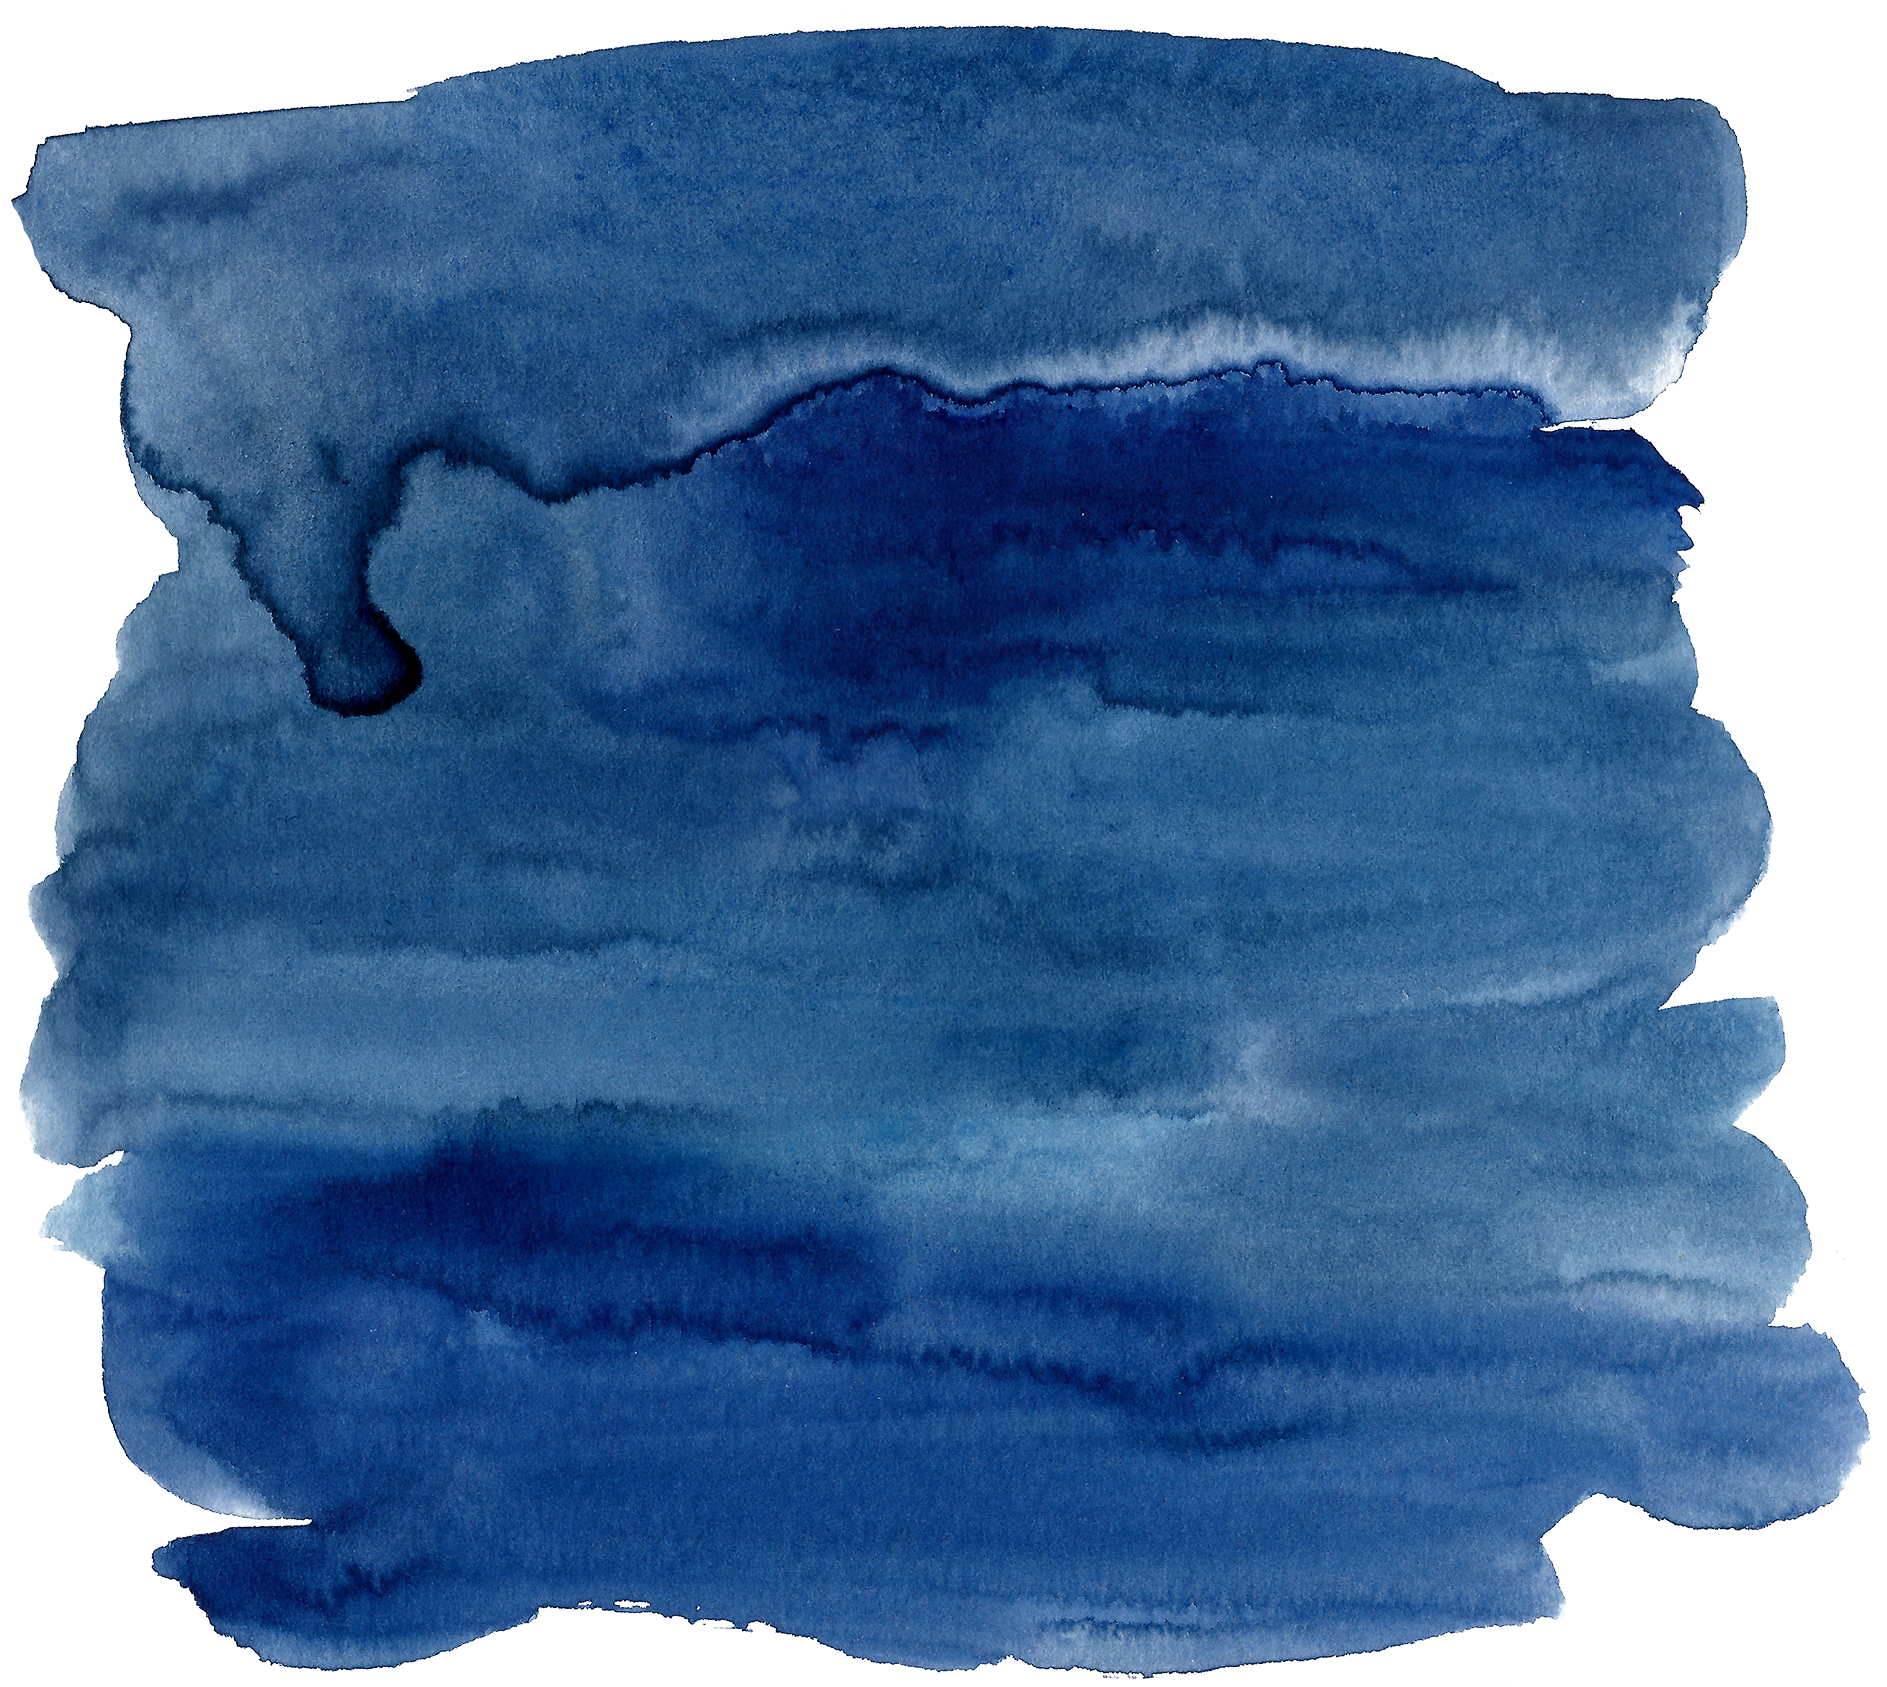
\includegraphics[width=1.07\paperwidth,height=1.07\paperheight]{FrontMatter/Cover/CoverBackground}}};


        %% we center all text
        \begin{center}

                %% The figure
                \vspace*{\fill}


                %% This can be used to set a foreground image
                %               - Ussually some tweaking with vertical space is needed to place it exactly
                \begin{figure}[H]
                        %        	\vspace*{-3.5cm}
                        \makebox[\linewidth]{
                                \scalebox{-1}[1]{\includegraphics[width=0.6\textwidth, clip, trim={0cm 0cm 0cm 0cm}]{FrontMatter/Cover/Cover}}
                        }
                        %        	\vspace*{1.0cm}
                \end{figure}



                %% Additional whitespace for ease of eye
                \vspace*{2\bigskipamount}


                %% Text color is changed for readability
                \color{white}

                %% Print the name of the author.
                {\makeatletter
                        \largetitlefont\Large\bfseries
                        \largetitlestyle\fontsize{24}{13cm}\selectfont Utrecht University
                        \makeatother}


                %% Additional whitespace for ease of eye
                \vspace*{2\bigskipamount}
        \end{center}


% \end{titlepage}

%% Print an overview of the layout
%\layout

\end{document}


